\section{Resoconto attività di verifica}
In questa sezione vengono descritti e analizzati gli esiti delle attività di verifica svolte su tutti i documenti che vengono consegnati nelle varie revisioni di avanzamento del progetto.
	\subsection{Revisione dei Requisiti}
		\subsubsection{Verifica della documentazione}
		Per la verifica della documentazione viene utilizzata la tecnica del \glock{walkthrough}, che ha portato all'individuazione di errori frequenti, insieme alla tecnica di \glock{inspection}, che mira a cercare gli errori più frequenti, come descritto nel documento \dext{norme di progetto v. 1.0.0}\footnote{sezione §3.4.4.1}
		\subsubsection{Leggibilità documenti}
		Nella tabella seguente vengono riportati gli indici di \glock{Gulpease} dei documenti finora stesi.
		\begin{center}
			\rowcolors{2}{white}{lightest-grayest}
			\begin{longtable}{|C{8cm}|C{4cm}|}
				\hline
				\rowcolor{lighter-grayer}
				\textbf{Documento} & \textbf{Indice di Gulpease} \\ 			
				\hline
				\endhead
				
				\hline
				Norme di Progetto v. 1.0.0 & 61 \\
				\hline
				Studio di Fattibilità v. 1.0.0 & 62 \\
				\hline
				Piano di Progetto v. 1.0.0 & 56 \\
				\hline
				Analisi dei Requisiti v. 1.0.0 & 58 \\
				\hline
				Piano di Qualifica v. 1.0.0 & 59 \\
				\hline
				Glossario v. 1.0.0 & 61 \\
				\hline
				Media verbali & 63 \\
				\hline
				
				\hiderowcolors
				\caption{Indice di Gulpease per ogni documento}		
			\end{longtable}	
		\end{center}
	\subsection{Periodo dalla Revisione dei Requisiti alla Revisione di Progettazione}
		\subsubsection{Accuratezza della pianificazione}
		\paragraph{Accuratezza della pianificazione per singolo ruolo}
		\begin{figure}[H]
	\centering
	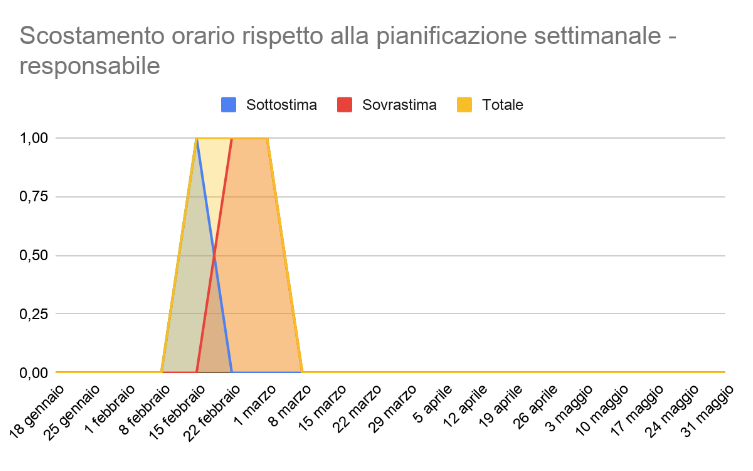
\includegraphics[width=10cm]{res/images/responsabile}
	\caption{Scostamento orario settimanale ruolo Responsabile}
	\label{fig:Scostamento orario settimanale ruolo Responsabile}
\end{figure}
\begin{figure}[H]
	\centering
	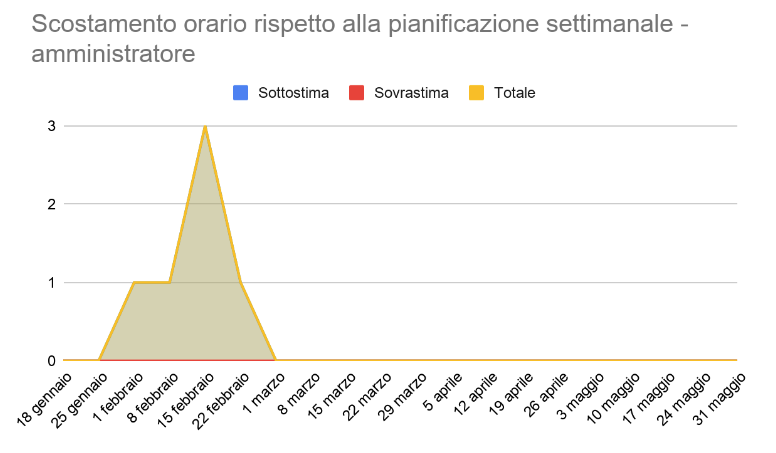
\includegraphics[width=10cm]{res/images/amministratore}
	\caption{Scostamento orario settimanale ruolo Amministratore}
	\label{fig:Scostamento orario settimanale ruolo Amministratore}
\end{figure}
\begin{figure}[H]
	\centering
	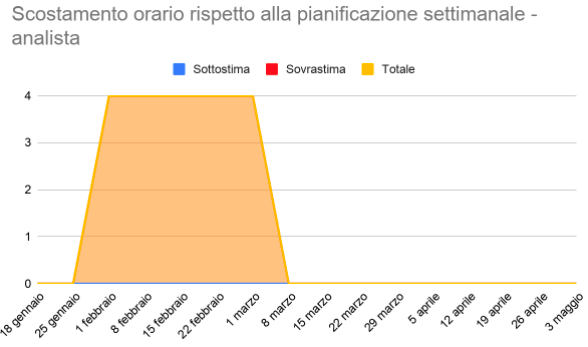
\includegraphics[width=10cm]{res/images/analista}
	\caption{Scostamento orario settimanale ruolo Analista}
	\label{fig:Scostamento orario settimanale ruolo Analista}
\end{figure}
\begin{figure}[H]
	\centering
	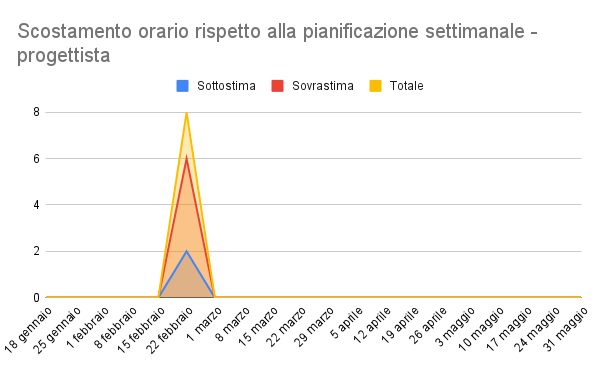
\includegraphics[width=10cm]{res/images/progettista}
	\caption{Scostamento orario settimanale ruolo Progettista}
	\label{fig:Scostamento orario settimanale ruolo Progettista}
\end{figure}
\begin{figure}[H]
	\centering
	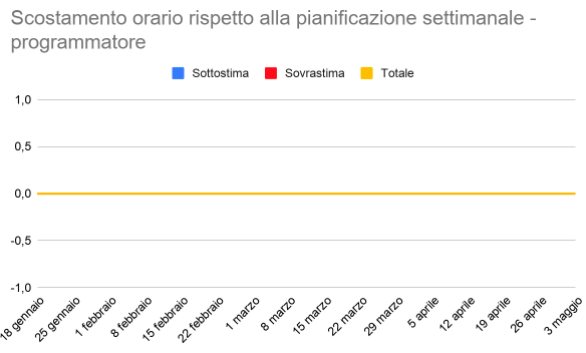
\includegraphics[width=10cm]{res/images/programmatore}
	\caption{Scostamento orario settimanale ruolo Programmatore}
	\label{fig:Scostamento orario settimanale ruolo Programmatore}
\end{figure}
\begin{figure}[H]
	\centering
	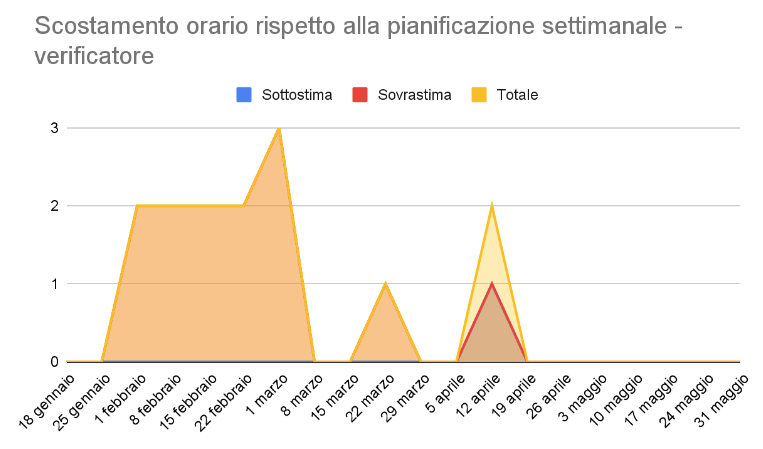
\includegraphics[width=10cm]{res/images/verificatore}
	\caption{Scostamento orario settimanale ruolo Verificatore}
	\label{fig:Scostamento orario settimanale ruolo Verificatore}
\end{figure}
\paragraph{Accuratezza della pianificazione per tutti i ruoli}
\begin{figure}[H]
	\centering
	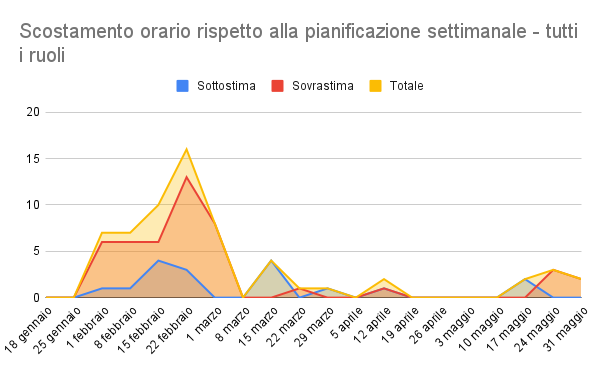
\includegraphics[width=10cm]{res/images/tutti}
	\caption{Scostamento orario settimanale per tutti i ruoli complessivamente}
	\label{fig:Scostamento orario settimanale per tutti i ruoli complessivamente}
\end{figure}